\documentclass[letterpaper,11pt]{article}

\usepackage[utf8x]{inputenc}
\usepackage{graphicx}
\usepackage{amsmath}
\usepackage{natbib}
\usepackage{setspace}
\usepackage{lscape}
\usepackage{longtable}
\usepackage{tabularx}
\usepackage{pdflscape}
\usepackage{geometry}
%\usepackage[
%singlelinecheck=false % <-- important
%]{caption}
\usepackage{wrapfig}

%opening
\newcommand{\cruiseID}{S275}
\title{\cruiseID\ Cruise Report}
\author{Benjamin Harden}

\geometry{
 letterpaper,
 left=20mm,
 top=20mm,
 right=20mm,
 bottom=20mm,
 footskip = 5mm
 }

%\textwidth=7.5in
%\textheight=10in
%oddsidemargin=.5cm
%\hoffset = -.5in
%\voffset = -.5in
\setlength{\parskip}{1em}


\begin{document}

\begin{titlepage}
	\centering
        \vspace*{.3cm}
	{\scshape\LARGE Cruise Report \par}
	{\scshape\Large \cruiseID : Sustainability in Polynesian Island Cultures and Ecosystems \par}
	\vspace{1.5cm}
	{\scshape\huge\bfseries Scientific Activities Undertaken Aboard the SSV Robert C. Seamans\par}
	\vspace{1cm}
        {\scshape\Large Pago Pago, American Samoa -- Neiafu, Tonga -- Nuku'alofa, Tonga -- Suva, Fiji -- Auckland, New Zealand \par}
        {\scshape\large 28  September -- 6 November, 2017\par}
        \vspace{1cm}        
        \includegraphics[height=0.4\textheight]{./images/S275_cover}\par
        \vspace{1cm}
	\large Sea Education Association, Woods Hole, Massachusetts
	\vfill
\end{titlepage}


\vspace*{\fill}
\noindent Citation: Harden, B.E., 2018. Final Report for S.E.A. Cruise \cruiseID . Sea Education Association, Woods Hole, MA 02543, USA. www.sea.edu.

\noindent\textbf{To obtain unpublished data, contact the SEA Data Archivist:}\\
Data Archivist\\
Sea Education Association\\
PO Box 6\\
Woods Hole, MA 02543\\
E-mail: data-archives@sea.edu\\

\clearpage
\listoffigures
\listoftables
\clearpage


\begin{table}[ht]
 \caption{\label{shipCompany} \cruiseID\ Ship's Company, \textit{SSV Robert C. Seamans}}\\
\\
\begin{tabular}{p{8cm} l}
 
  \vspace*{0.2cm}
  \textbf{Faculty} \\
  \hline
  Jay Amster & Captain\\
  Jeff Wescott & Chief Anthropologist\\
  Benjamin Harden & Chief Scientist\\
\\
  \textbf{Crew}\\
  \hline
  Alison Taylor  & Chief Mate\\
  Rebecca Jackson & 2nd Mate\\
  Tristan Feldman & 3rd Mate\\
  Brittany Mauer & 1st Assistant Scientist\\
  Erin Adams & 2nd Assistant Scientist\\
  Erin Houlihan & 3rd Assistant Scientist\\
  Edward Flemming & Chief Engineer\\
  Michael Rigney & Assistant Engineer\\
  Sabrina Hutchinson & Steward\\
  Christian Letourneau & Steward-in-training\\
\\
  \textbf{Observers}\\
  \hline
  Yumi Asagi (Tonga) & Pago Pago -- Suva\\
  Vani Koroisamanunu (Fiji) & Nuku'alofa -- Auckland\\
\\
  \textbf{Students}\\
  \hline
  Mary Elizabeth Benton &	Sewanee: The University of the South \\
  Nikkol Blair	& Colorado College \\
  Graeme Brown&	Colby College \\
  Claire Caputi &	Colby College\\
  Amanda Carreau&	University of Massachusetts, Amherst\\
  Hannah Chiu &	Pitzer College\\
  Alison Derevensky&	Macaulay Honors at CUNY Brooklyn College\\
  Anna Gaskill	&Wellesley College\\
  Amy Green&	Boston University\\
  Katharine Hall &	Sewanee: The University of the South\\
  Katherine Hodge &	University of Chicago\\
  Arya Jemal &	Swarthmore College \\
  Joshua Jolly &	University of Denver\\
  Kellen McAuliffe&	Colgate University\\
  Faith McKenna&	University of Denver\\
  Henry Oliva&	Colby College \\
  Flannery Raabe&	Oberlin College\\
  Alessandra Rella&	Franklin and Marshall College \\
  Noah Robiner&	Carleton College\\
  Sierra Schmitz&	American University\\
  Sarah Towne&	Cornell University\\

\end{tabular}
\end{table}

\clearpage
\section*{Data Description}

\begin{wrapfigure}{R}{0.5\linewidth}
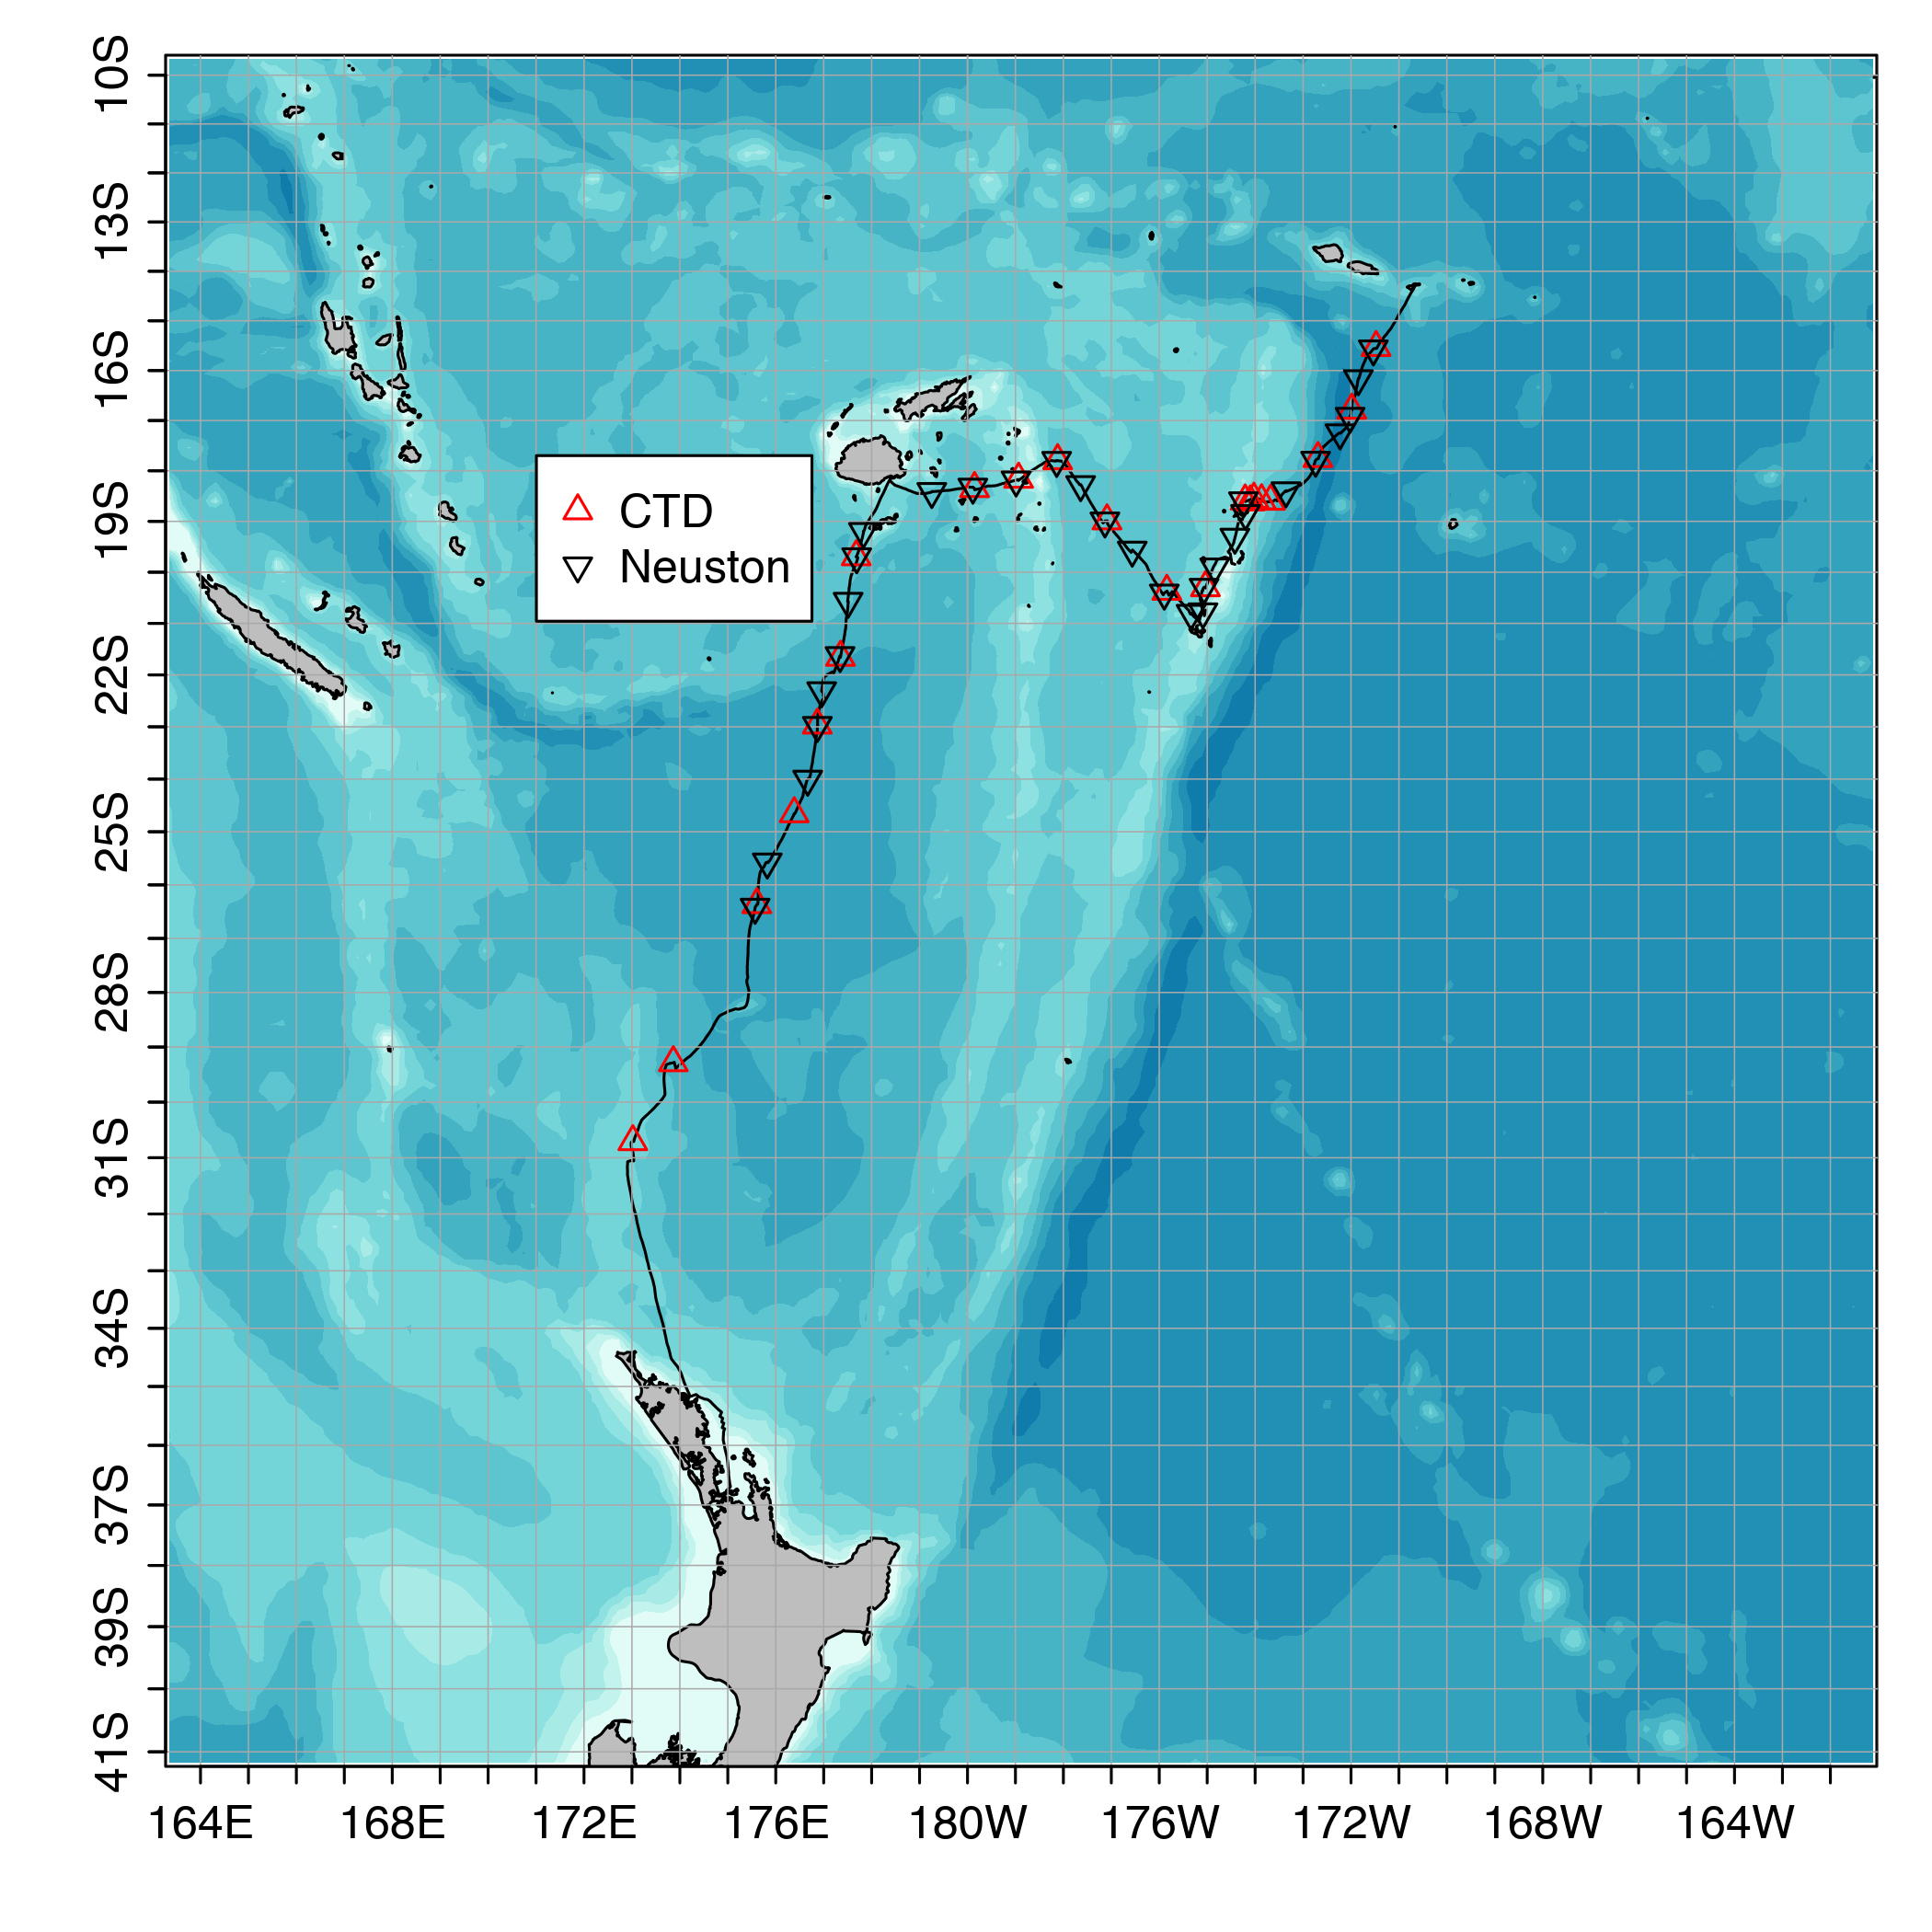
\includegraphics[width=\linewidth]{./plots/S275_cruiseTrack.png}
\caption[The \cruiseID\ cruise track]{The \cruiseID\ cruise track from hourly GPS data. Overlaid are the locations of the CTD/Hydrocast and Neuston Stations.}
\label{cruiseTrack}
\end{wrapfigure}

This report summarizes the science activities aboard the \textit{SSV Robert C. Seamans} during the Sea Education Association's Fall 2017 semester ''Sustainability in Polynesian Island Cultures and Ecosystems'' (SPICE), cruise S275. This cruise departed Pago Pago, in American Samoa on 28th September 2017 and concluded in Auckland on 6th November 2017. En route, the Seamans had port calls in Neiafu in the Vava'u island group of Tonga (4--7 Oct), in Nuku'alofa the Tongan Capital in the southern Tongatapu island group (11--14th Oct), and in Suva, Fiji (19--23 Oct). On the leg between American Samoa and the Vava'u, we crossed the international date line. The 1st October was skipped and our clocks went from midnight at the end of the 30th September to midnight at the end of the 1st October.

The cruise track spanned a range of oceanographic environments. We transited from the the tropics in American Samoa to the temperate mid-latitudes around New Zealand's North Island, crossing the western side of the south Pacific Gyre en route. We also had the opportunity to sampled across the transition from near-shore to open ocean as we transited through the Tongan and Fijian region.

The 21 students of S275 were all active and responsible for data collection in the lab. Although this particular semester program is science-lite in it's focus, students all undertook small research projects pertaining to the ocean data collected. In addition to investigations of physical, chemical and biological properties along the whole cruise track, the two addional key topics of investigation were the Island Mass Effect and Ocean Soundscapes.

To accomplish our science goals our sampling plan included:

\begin{itemize}
  \item A standard SEA portfolio of noon CTD casts, twice-daily Neuston tows, and continuous measurements from ADCP, Chirp and flow-through system;
 \item Surface and subsurface samples for extracted chlorophyll-a, Nitrate, Phosphate and pH. This included high-resolution surface stations approaching and/or leaving port to probe run-off. We also conducted hydrocasts upstream and downstream of islands to investigate island upwelling.
 \item Noon hydrophone deployments (outlined below).
 \item Day-time, hourly 6-minute observations of fauna and debris.
 \item Occasional midnight CTD casts.
 \item Occasional midnight Meter-Net tows to approximately 200 m.
 \item Occasional RBR-CTD towed deployments (outlined below).
 \item Filtering for Microplastics from water samples.
\end{itemize} 

The winds for this cruise were predominantly from an easterly direction (Figure \ref{winds}) and presented little in the way of obstruction to our movement along the cruise track. The easterlies were maintained all the way to New Zealand. In the previous year (S269), the winds had been from a more south-easterly direction before transitioning to westerlies south of 30$^{\circ}$S. As a result, the cruise track heading southward from Fiji this year was much mire direct. S269's cruise track tended more westward before returning eastward to New Zealand. For the second half of the long passage to New Zealand, the winds were sustained strong with large seas. As a result, we undertook limited sampling south of 30$^{\circ}$S, instead opting to make the most of the winds in moving us towards our destination.

This summary of the data is not meant to be exhaustive; lengthy data sets from, for example, ADCP, CTDs, or CHIRP, have not been included in their entirety. All data is available and can be requested from the SEA data archivist.

-- Ben Harden, Chief Scientist, \cruiseID


\subsection*{Hydrophone Deployments}
Part of our standard sampling during this cruise was noon hydrophone deployments. This was motivated partly by our proximity to humpback whale breeding grounds in Tonga and partly by a desire from SEA faculty to expand our capabilities in this area given our relatively quiet vessels.

The hydrophone was streamed from the port-side of the quarter deck while the Seamans was hove-to. Our standard protecol was to make 30-minute recordings on a TASCAM audio recorder. However, some deployments varied in length. During the hydrophone deployment we undertook visual surveys of ships and marine mammals.

Two notable deployments were stations 16 and 38 on the 8 Oct and 27 Oct respectively.

During station 16 we were in the shallow breeding grounds of humpback whales in Tonga. During the recording (which was approximately 1hr20m long) we saw numerous whales displaying a range of behaviours. This recording is our best record of humpback whale song along our cruise track.

During station 38 we conducted an experiment into the soundscape of the Seamans itself. We systematically secured machinery aboard the ship to isolate the sounds that each produced. This included a short period (approximately 30 seconds) of black-shop when all engineering equipment was secured. The meta data for this experiment is recorded in the SEA Archive.

\subsection*{RBR-CTD towed deployments}

We experimented with deploying the RBR-CTD on a towable wing during this cruise. This was deployed from the BT winch on the starboard quarter and was towed in a saw-tooth configuration while the ship was in transit. The goal of this deployment was to investigate small-scale structures in the vertical and horizontal around island regions that could be indicative of eddy shedding or localized upwelling.

We deployed four times, once in the open ocean between American Samoa and Tonga, twice around the island group of Vava'u (one upstream, one downstream) and once south of Vava'u as we moved from the shallow shelf region (approx. 100m) to the deep ocean. An example is presented in Figure \ref{CTD_RBR}.

The salinity data from these casts is suspect in comparison with Seabird CTD data at nearby casts (Figure \ref{CTD_RBR}). This is not necessarily surprising. The RBR module is an older model made before the company moved to improve the flow through the induction cell. The flow over the towable wing might also be mixing and trapping water pockets thereby also creating issues with the data collected. The data below is presented as-is and should be considered not quality controlled.

\subsection*{Additional Data Notes}

\begin{itemize}
 \item One event file was maintained for the duration of the cruise (ELG 002)
 \item The author suspects that the ADCP data export by the onboard system and recorded in the ODV text files in our archive is probably not accurate. There are occasions when the current direction appears correlated to the ships heading and so can't be considered physical. This needs further investigation and is the reason why no ADCP data is shown in this report. ADCP data from the SEA archive should be considered in this light also.
 \item Please request the end of cruise report for full technical details of ship science operations.
\end{itemize}


\clearpage
\subsection*{Figures}

\begin{figure}[h]
\centering
\includegraphics[width=0.9\linewidth]{./plots/\cruiseID _CTD_section.png}
\caption[CTD Section running along the \cruiseID\ cruise track]{CTD Section running along the \cruiseID\ cruise track - left: map of stations; top right: temperature; middle right: Salinity; bottom right: Potential Density. Select station numbers are shown with red circles in left panel. All profile locations are shown with gray lines in panels on right with select stations numbered. See Tables \ref{hydrowork} and \ref{ctdwork} for full cast details. Concentrated casts around Vava'u in northern Tonga were an attempt to investigate the Island Mass Effect around the island.}
\label{CTD_section}
\end{figure}

\begin{figure}[ht]
\centering
\includegraphics[width=\linewidth]{./plots/\cruiseID _CTD_section_2.png}
\caption[Auxiliary CTD data running along the \cruiseID\ cruise track]{As Figure \ref{CTD_section} but for auxiliary CTD data running along the \cruiseID\ cruise track. Top: Chlorophyll-a Fluormeter. Bottom: Oxygen Concentration.}
\label{CTD_section_2}
\end{figure}

\begin{figure}[ht]
\centering
\includegraphics[width=\linewidth]{./plots/\cruiseID _009_RBR_grid.png}
\caption[CTD data from RBR Tow-Yo]{Example of one Tow-Yo deployment using an RBR CTD towed from the BT winch upstream of Vava'u in northern Tonga. Panels as Figure \ref{CTD_section}. CTD stations 8 and 10 (Seabird CTDs) were undertaken at either end of the RBR tow period and are appended to the record for the sake of this figure. Only the downcast of the RBR deployment were used for this plot (of which there were 8). As can be seen, the Seabird CTD data doesn't necessarily match well with that of the RBR. There were three more deployments of the RBR in this manner.}
\label{CTD_RBR}
\end{figure}


\begin{figure}[t]
\centering
\includegraphics[width=\linewidth]{./plots/\cruiseID _hydrowork.png}
\caption[Hydrocast summary along \cruiseID\ cruise track]{Hydrocast data from the complete /cruiseID/ cruise track. Left: Map of all hydrocast locations. Top right: Extracted Chlorophyll-a (0.45um filter; mg/L); middle right: Nitrate Concentration (uM), bottom right: Phosphate Concentration (uM). Concentrated sampling around Vava'u in northern Tonga was an attempt to detect signatures of upwelling due to the Island Mass Effect.}
\label{hydrowork}
\end{figure}

\begin{figure}[t]
\centering
\includegraphics[width=\linewidth]{./plots/\cruiseID _flowthrough.png}
\caption[Underway flow-through data from the \cruiseID\ cruise track]{Underway flow-through data from the \cruiseID\ cruise track. From top left: Surface water temperature ($^{\circ}$C), salinity, chlorophyll fluorescence (volts) and CDOM fluorescence (volts) as measured by flow through system sensors.}
\label{hourly}
\end{figure}

\begin{figure}[t]
\centering
\includegraphics[width=\linewidth]{./plots/\cruiseID _surfStat.png}
\caption[Surface Station data from along \cruiseID\ cruise track]{Surface Station data from along \cruiseID\ cruise track. From top left: Surface water nitrate concentration (uM), phosphate concentration (uM), chlorophyll concentration (0.45um filter; mg/L), and pH as measured by laboratory analyses on discrete surface station water samples. See Table \ref{surfsamp} for full station details.}
\label{surfstat}
\end{figure}

\begin{figure}[t]
\centering
\includegraphics[width=\linewidth]{./plots/\cruiseID _winds.png}
\caption[Wind vector summary]{Wind speed and direction for the \cruiseID\ cruise track, as measured by the ship’s anemometer. Lines indicate direction that the winds are flowing towards.}
\label{winds}
\end{figure}

\begin{figure}[t]
\centering
\includegraphics[width=\linewidth]{./plots/\cruiseID _biomass.png}
\caption[Zooplankton biomass]{Total zooplankton biomass ($\mu L/m^2$) for neuston tows on cruise \cruiseID. Grey circles are night time tows and white are for day time.}
\label{biomass}
\end{figure}

\begin{figure}[t]
\centering
\includegraphics[width=\linewidth]{./plots/\cruiseID _biodiversity.png}
\caption[Zooplankton Biodiversity]{Total zooplankton biodiversity (Shannon-Wiener Index) for neuston tows on cruise \cruiseID\. Data is computed from standard SEA 100 count methodology. Grey circles are night time tows and white are for day time.}
\label{biodiversity}
\end{figure}

\begin{figure}[t]
\centering
\includegraphics[width=\linewidth]{./plots/\cruiseID _plastics.png}
\caption[Plastic Distribution]{Total number of plastic pieces found in neuston tows on cruise \cruiseID.}
\label{plastics}
\end{figure}



\clearpage
\begin{landscape}
\subsection*{Tables}

\fontsize{10}{12}\selectfont


\input{./tables/\cruiseID _StationSummary.tex}
\noindent Notes: abbreviations for oceanographic equipment deployments are: NT – neuston tow; MN – 1-meter or 2-meter net (oblique tow); PN – phytoplankton net; HC – hydrocast with 12 Niskin bottles, CTD and optical instrumentation; CTD – free CTD with no water samples; RBR - RBR type free CTD with no water samples, SG – shipek grab, SS - Surface Station.


\clearpage

\input{./tables/\cruiseID _Hydrowork.tex}
\noindent Notes: all hydrocasts gathered data from a SeaBird 19PlusV2 CTD (S/N 4043) and three auxiliary instruments (Seapoint Chlorophyll fluorometer (S/N SCF-3149), SeaBird Dissolved Oxygen sensor (model 43; S/N 1518), and Biospherical Instruments/SeaBird PAR sensor (S/N 4179). Extracted chlorophyll-a samples were filtered through 0.45 $\mu$m filters and measured with a Turner Designs Model 10-AU fluorometer. Seawater pH was determined using m-cresol purple indicator dye and spectrophotometry. Nutrients (PO4 and NO3) were assessed with colorometric spectrophotometry. A blank space indicates that no sample was collected for that analysis. DNF indicates a bottle that Did Not Fire.

\clearpage
\input{./tables/\cruiseID _Ctdwork.tex}

\clearpage
\input{./tables/\cruiseID _surfsamp.tex}
\noindent Notes: extracted chlorophyll-a samples were filtered through 0.45 $\mu$m filters and measured with a Turner Designs Model 10-AU fluorometer. Seawater pH was determined using m-cresol purple indicator dye and spectrophotometry. Nutrients (PO4 and NO3) were assessed with colorometric spectrophotometry.

\clearpage
\input{./tables/\cruiseID _Neuston_1.tex}
\noindent Notes: tow area calculated using distance (meters) between successive minutes' GPS positions. Neuston net opening 1.0m wide by 0.5m tall, with a 333 $\mu$m mesh net. Zooplankton density recorded as wet volume displacement per tow area ($mL/m^2$).\\

\clearpage
\input{./tables/\cruiseID _Neuston_2.tex}
\noindent Notes: Eel larvae (leptocephali - lept), spiny lobster larvae (phyllosoma - phyl), marine water striders (halobates - halo) and Lantern fish (myctophids - myct) sorted from net contents and counted. Micronekton and gelatinous micronekton removed using a 333 $\mu$m mesh sieve; biovolume (ml) recorded. Qualitative descriptions of micronekton removed from zooplankton biomass are available. Floating plastic and tar removed from net contents, sorted and recorded as numbers collected per tow.

\clearpage
\input{./tables/\cruiseID _Neuston_100Count_1.tex}
\noindent Notes: abbreviations for zooplankton categories: Cnid – cnidarian medusa; Siph – siphonophore bracts and floats; Cten – ctenophores; Pter – pteropods; Nud - nudibranchs; Other Snail – pelagic snails; Ceph – cephalopods; Poly – polychaetes; Chaet – chaetognaths; Cop – copepods; Gam Amp – gammarid amphipods; Hyp Amp – hyperiid amphipods; Crab (larv) – Crab zoea and megalops.

\clearpage
\input{./tables/\cruiseID _Neuston_100Count_2.tex}
\noindent Notes: abbreviations for zooplankton categories: Shr Larv, – shrimp larval stage; Lob Larv. – lobster larval stage; Mys – mysids; Euph – euphausiids; Stom Larv. – stomatopod larval stage; Ost – ostracods; Clad – cladocerans; Iso – isopods; Salp – salps and doliolids; Fish Larv. - larval fish; Other - Other categories not listed individually in Tables \ref{100count1} or \ref{100count2}.



\end{landscape}

\end{document}